\documentclass[11pt,a4paper]{article}

\usepackage[utf8]{inputenc}
\usepackage[spanish,es-tabla]{babel}
\usepackage[margin=2.5cm]{geometry}
\usepackage{graphicx}
\usepackage{booktabs}
\usepackage{amsmath}
\usepackage{siunitx}
\usepackage{float}
\usepackage[hidelinks]{hyperref}
\usepackage{caption}
\captionsetup{font=small,labelfont=bf}

\sisetup{output-decimal-marker={,},group-separator={\,},group-minimum-digits=4}

% Las figuras y tablas se copian a report/figs y report/tabs por src/figures.py,
% de modo que esta carpeta es autocontenida (subir tal cual a Overleaf).
\graphicspath{{figs/}{../data/outputs/figs/}}
\newcommand{\tab}[1]{\InputIfFileExists{tabs/#1}{}{\input{../data/outputs/tabs/#1}}}

\title{\textbf{Accesibilidad vial a servicios de emergencia resolutivos\\
en Lambayeque, Apur\'imac y Amazonas}\\[0.3em]
\large An\'alisis geoespacial, m\'etricas de cobertura y desigualdad}
\author{Karelys S. Collazos \\
\small Data Science with Python --- HW\_02\_202602 --- \texttt{d2cml-ai/Data-Science-Python} \#186}
\date{\today}

\begin{document}
\maketitle

\begin{abstract}
\noindent
La \emph{hora dorada} en medicina de emergencia postula que la probabilidad de
supervivencia cae de forma marcada si el paciente no recibe atenci\'on
resolutiva en los primeros 60 minutos. Este trabajo estima, para
\num{8781} centros poblados de tres departamentos que representan la costa
(Lambayeque), la sierra (Apur\'imac) y la selva (Amazonas), el tiempo de viaje
\emph{por carretera} hasta el establecimiento de salud resolutivo m\'as cercano
(categor\'ia II-1 o superior). Se construye una matriz origen--destino de
\num{342} mil pares con OSRM, se ponderan los indicadores por poblaci\'on del
Censo 2017 y se analiza la cobertura, la desigualdad (Gini) y su relaci\'on con
altitud y pobreza distrital. \textbf{Resultado principal:} el
\SI{16.6}{\percent} de la poblaci\'on queda fuera de la hora dorada, con un Gini
de acceso de \num{0.66} y un gradiente claro con la pobreza: el cuartil de
distritos m\'as pobres tarda del orden de siete veces m\'as que el menos pobre.
\end{abstract}

\section{Introducci\'on y planteamiento del problema}

En medicina de emergencia, la \emph{hora dorada} designa el intervalo tras un
traumatismo o evento cr\'itico durante el cual la atenci\'on resolutiva
--- cirug\'ia, cuidados intensivos, transfusi\'on --- tiene el mayor impacto
sobre la supervivencia. En el sistema peruano, esa capacidad se concentra en
los establecimientos de categor\'ia II-1 y superiores; los de primer nivel
(I-1 a I-4) derivan. El tiempo que tarda un paciente en llegar a un
establecimiento resolutivo es, por tanto, un indicador directo de equidad
territorial en salud.

La distancia en l\'inea recta a un hospital subestima sistem\'aticamente ese
tiempo, sobre todo en zonas andinas y amaz\'onicas donde la red vial es
sinuosa, discontinua o inexistente y el relieve impone grandes rodeos. Medir
el \emph{tiempo de viaje por carretera} --- y no la distancia --- es lo que
permite localizar las brechas reales de cobertura.

La pregunta de investigaci\'on es: \emph{¿qu\'e fracci\'on de la poblaci\'on de
cada regi\'on natural puede alcanzar un establecimiento resolutivo dentro de la
hora dorada, y c\'omo se distribuye esa carencia entre territorios urbanos y
rurales, de mayor y menor altitud, y de mayor y menor pobreza?}

Objetivos: (i) construir \emph{datasets} geoespaciales validados de oferta
(establecimientos II-1+) y demanda (centros poblados con poblaci\'on); (ii)
calcular tiempos de viaje viales origen--destino con un motor de ruteo; (iii)
derivar indicadores de cobertura y de desigualdad ponderados por poblaci\'on, y
cruzarlos con altitud y pobreza; (iv) identificar los distritos con mayor
brecha y ofrecer un panel que permita simular intervenciones. El estudio se
acota a tres departamentos que representan las tres regiones naturales:
Lambayeque (costa), Apur\'imac (sierra) y Amazonas (selva).

\section{Datos}

\subsection{Fuentes}
\begin{itemize}
  \item \textbf{Oferta.} RENIPRESS (SUSALUD), padr\'on de agosto de 2026.
        Se retienen los establecimientos \textsc{activo}s de categor\'ia
        II-1, II-2, II-E, III-1, III-2 o III-E.
  \item \textbf{Demanda.} Centros poblados del Censo 2017 (INEI, distribuci\'on
        geogpsperu) con poblaci\'on, altitud, categor\'ia y coordenadas.
  \item \textbf{L\'imites distritales.} Cartograf\'ia distrital (l\'imites INEI).
  \item \textbf{Contexto.} Pobreza monetaria e IDH distrital
        (INEI\,/\,PNUD, v\'ia \texttt{ubigeo-peru-aumentado}).
  \item \textbf{Red vial.} OpenStreetMap, servida por OSRM.
\end{itemize}

\subsection{Validaci\'on y control de calidad}
Cada registro pasa por un conjunto de reglas que producen banderas
\texttt{qc\_*} sin eliminar la fila; el an\'alisis posterior filtra por ellas
pero conserva la trazabilidad completa. Las reglas son:

\begin{itemize}
  \item \texttt{coord\_faltante} / \texttt{isla\_cero}: coordenadas ausentes o
        pr\'acticamente nulas ($|\text{lat}|,|\text{lon}|<0{,}01$), error de
        captura habitual.
  \item \texttt{fuera\_de\_peru} / \texttt{latlon\_invertida}: el punto cae
        fuera del \emph{bounding box} nacional, o s\'olo entra si se
        intercambian latitud y longitud.
  \item \texttt{depto\_fuera\_ambito}: el UBIGEO no corresponde a ninguno de los
        tres departamentos.
  \item \texttt{duplicado\_codigo} / \texttt{duplicado\_espacial}: c\'odigo
        repetido, o dos puntos a menos de \SI{50}{m} dentro del mismo distrito.
  \item \texttt{categoria\_invalida} / \texttt{no\_activo} (s\'olo oferta): la
        categor\'ia no sigue el patr\'on \texttt{I-1}\ldots\texttt{III-E}
        (incluye el valor literal \texttt{"0"}), o el establecimiento no est\'a
        \textsc{activo}.
  \item \texttt{poblacion\_no\_positiva} (s\'olo demanda): centro poblado con
        poblaci\'on censada nula.
\end{itemize}

Las Tablas~\ref{tab:calidad-oferta} y~\ref{tab:calidad-demanda} resumen los
resultados sobre los datos del \'ambito de estudio.

\tab{tab_calidad_oferta.tex}
\tab{tab_calidad_demanda.tex}

Los hallazgos m\'as relevantes: cerca de una cuarta parte de los
establecimientos del \'ambito figura sin coordenadas y otra cuarta parte con
categor\'ia no v\'alida, lo que reduce de forma sustancial la oferta utilizable
y obliga a documentar expl\'icitamente qu\'e se descarta y por qu\'e. En torno
al \SI{19}{\percent} aparece como no activo. Los duplicados espaciales
(\textasciitilde\SI{19}{\percent}) corresponden en su mayor\'ia a
re-registros del mismo establecimiento con ligeras variaciones de coordenada.
En la demanda, un \SI{17}{\percent} de los centros poblados tiene poblaci\'on
censada cero (localidades estacionales o despobladas): se conservan con peso
nulo, no se eliminan. Un incidente de calidad motiv\'o un cambio de \'ambito:
la capa de centros poblados de \textbf{Tumbes} (primera opci\'on de costa)
lleg\'o, en las dos variantes disponibles de la fuente, sin c\'odigo ni
poblaci\'on; se sustituy\'o por \textbf{Lambayeque}, cuya capa s\'i trae
poblaci\'on a nivel de centro poblado. Con el \'ambito final, la cobertura de
poblaci\'on es del \SI{100}{\percent} y no se aplica ninguna imputaci\'on.

\section{Metodolog\'ia}

\subsection{Ruteo y matriz origen--destino}
El conjunto de demanda son \num{8781} centros poblados v\'alidos; la oferta,
\num{39} establecimientos resolutivos activos. La matriz origen--destino
completa tiene por tanto $\num{8781}\times\num{39}=\num{342459}$ pares por
perfil. Cada par se resuelve con el servicio \texttt{/table} de OSRM (servidor
p\'ublico \texttt{router.project-osrm.org}), que devuelve simult\'aneamente
\emph{duraci\'on} y \emph{distancia} de conducci\'on por la red de
OpenStreetMap. Las peticiones se agrupan en lotes de hasta 100 coordenadas
(l\'imite del servidor) fijando los \num{39} establecimientos como
\emph{destinos} y hasta \num{61} centros poblados como \emph{or\'igenes} por
petici\'on, de modo que toda la matriz se cubre en unas 150 llamadas. Los
resultados se guardan en una cach\'e SQLite indexada por
\texttt{(ccpp\_id, facility\_id)}, lo que hace la ejecuci\'on reanudable y
permite reconstruir la matriz sin volver a consultar el servicio. El
\SI{100}{\percent} de los pares obtuvo ruta real.

Para pares eventualmente sin ruta (componentes desconectadas de la red, algo
frecuente en zonas amaz\'onicas sin v\'ias mapeadas) se define un
\emph{fallback} expl\'icito: $t = d_{\text{haversine}}\cdot \kappa / v$, con
factor de rodeo $\kappa=1{,}3$ y velocidad media $v$ del perfil. Es una cota
inferior --- asume trayecto directo --- y se marca en la columna
\texttt{source} para poder cuantificar su peso; en este estudio no fue
necesario.

El perfil \emph{caminando} se deriva de la distancia vial de OSRM a
\num{4.5}~km/h, ya que el servidor p\'ublico no expone perfil peatonal.
Es una aproximaci\'on conservadora (un peat\'on puede tomar atajos que un
veh\'iculo no) y se reporta \'unicamente como referencia comparativa frente a
la conducci\'on.

Se implement\'o y evalu\'o un motor alternativo enteramente local
(\texttt{osmnx} para descargar el grafo vial de los tres departamentos y
\texttt{networkx} para los caminos m\'inimos con Dijkstra desde cada
establecimiento). Se descart\'o como motor principal porque la descarga del
grafo desde la API de Overpass se subdivide en \textasciitilde170 subconsultas
para un \'area de esa magnitud y agota reiteradamente el tiempo de espera. El
c\'odigo permanece en el repositorio y puede activarse con
\texttt{routing.engine: osmnx} en \texttt{config.md}.

\subsection{M\'etricas}
Para cada centro poblado $i$ se toma el tiempo m\'inimo
$t_i=\min_j t_{ij}$ al conjunto de establecimientos $j$. Con poblaci\'on $w_i$:
\begin{itemize}
  \item \textbf{Cobertura} por bandas: \% de $\sum w_i$ con $t_i\le\{30,60,120\}$ min.
  \item \textbf{Tiempo medio ponderado} $\bar t = \sum w_i t_i / \sum w_i$.
  \item \textbf{Desigualdad}: Gini ponderado del vector $\{t_i\}$,
  \begin{equation}
    G = 1 - \frac{\sum_{k} (C_k + C_{k-1})\,(W_k - W_{k-1})}{C_n},\quad
    C_k = \!\!\sum_{m\le k}\! w_m t_m,\ \ W_k=\!\!\sum_{m\le k}\! w_m,
  \end{equation}
  con los $i$ ordenados por $t_i$ ascendente.
  \item \textbf{Cruces}: $\bar t$ por \'ambito urbano/rural, por tercil de
        altitud y por cuartil de pobreza distrital; correlaci\'on de $t_i$ con
        \% de pobreza e IDH.
\end{itemize}
El pipeline incluye una rutina de imputaci\'on para centros poblados sin
poblaci\'on (reparto del total distrital seg\'un la categor\'ia del centro
poblado), pensada para el caso Tumbes; con el \'ambito final (Lambayeque,
Apur\'imac, Amazonas) todos los centros poblados traen poblaci\'on del Censo
2017 y la imputaci\'on no se activa.

\subsection{Panel interactivo}
Los resultados se explotan en un panel \texttt{Streamlit} que funciona sin
conexi\'on a partir de los artefactos precomputados (matriz O--D y agregados
distritales versionados en el repositorio). Adem\'as de la cabecera de
indicadores, el \emph{choropleth} distrital y la distribuci\'on del tiempo de
acceso, incorpora un \textbf{simulador de escenarios} con dos modos: (i)
\emph{cerrar} uno o varios establecimientos y recalcular al vuelo el tiempo
m\'inimo de cada centro poblado a partir de la matriz --- lo que revela la
contribuci\'on de cada hospital a la cobertura ---, y (ii) \emph{a\~nadir} un
establecimiento resolutivo hipot\'etico en un distrito, estimando el efecto con
distancia directa. El panel muestra en tiempo real el cambio en el porcentaje
de poblaci\'on fuera de la hora dorada respecto a la situaci\'on actual.

\section{Resultados}

\begin{figure}[H]
  \centering
  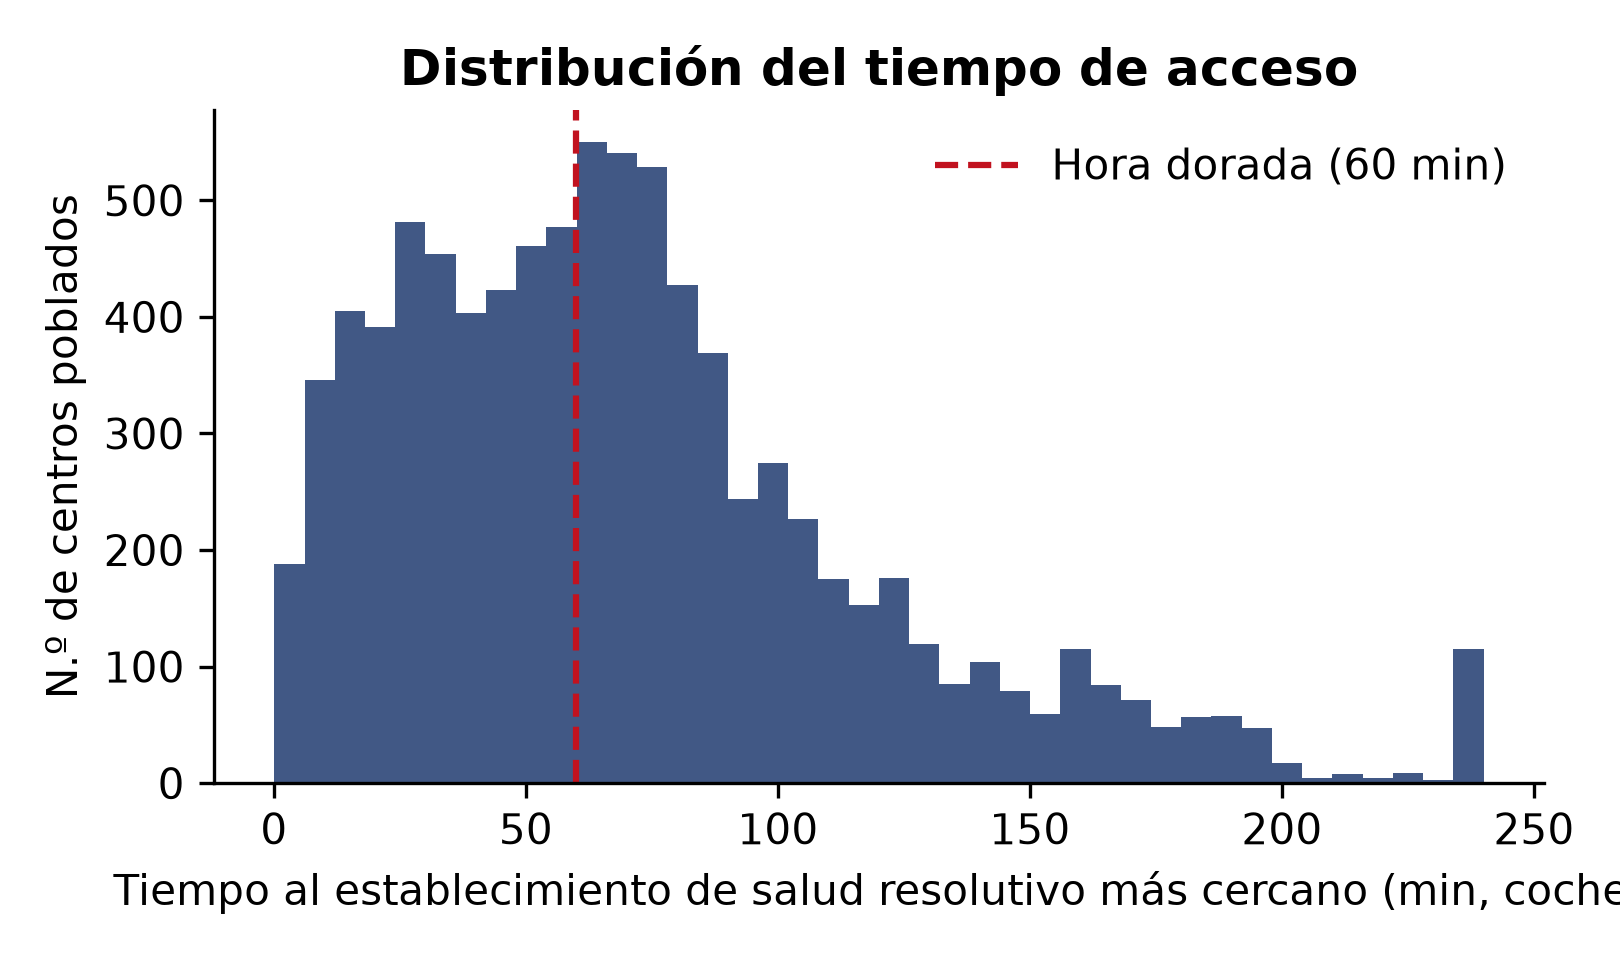
\includegraphics[width=0.72\linewidth]{fig_hist_acceso.png}
  \caption{Distribuci\'on del tiempo de acceso al hospital resolutivo m\'as
  cercano (conducci\'on). La l\'inea marca la hora dorada.}
  \label{fig:hist}
\end{figure}

\begin{figure}[H]
  \centering
  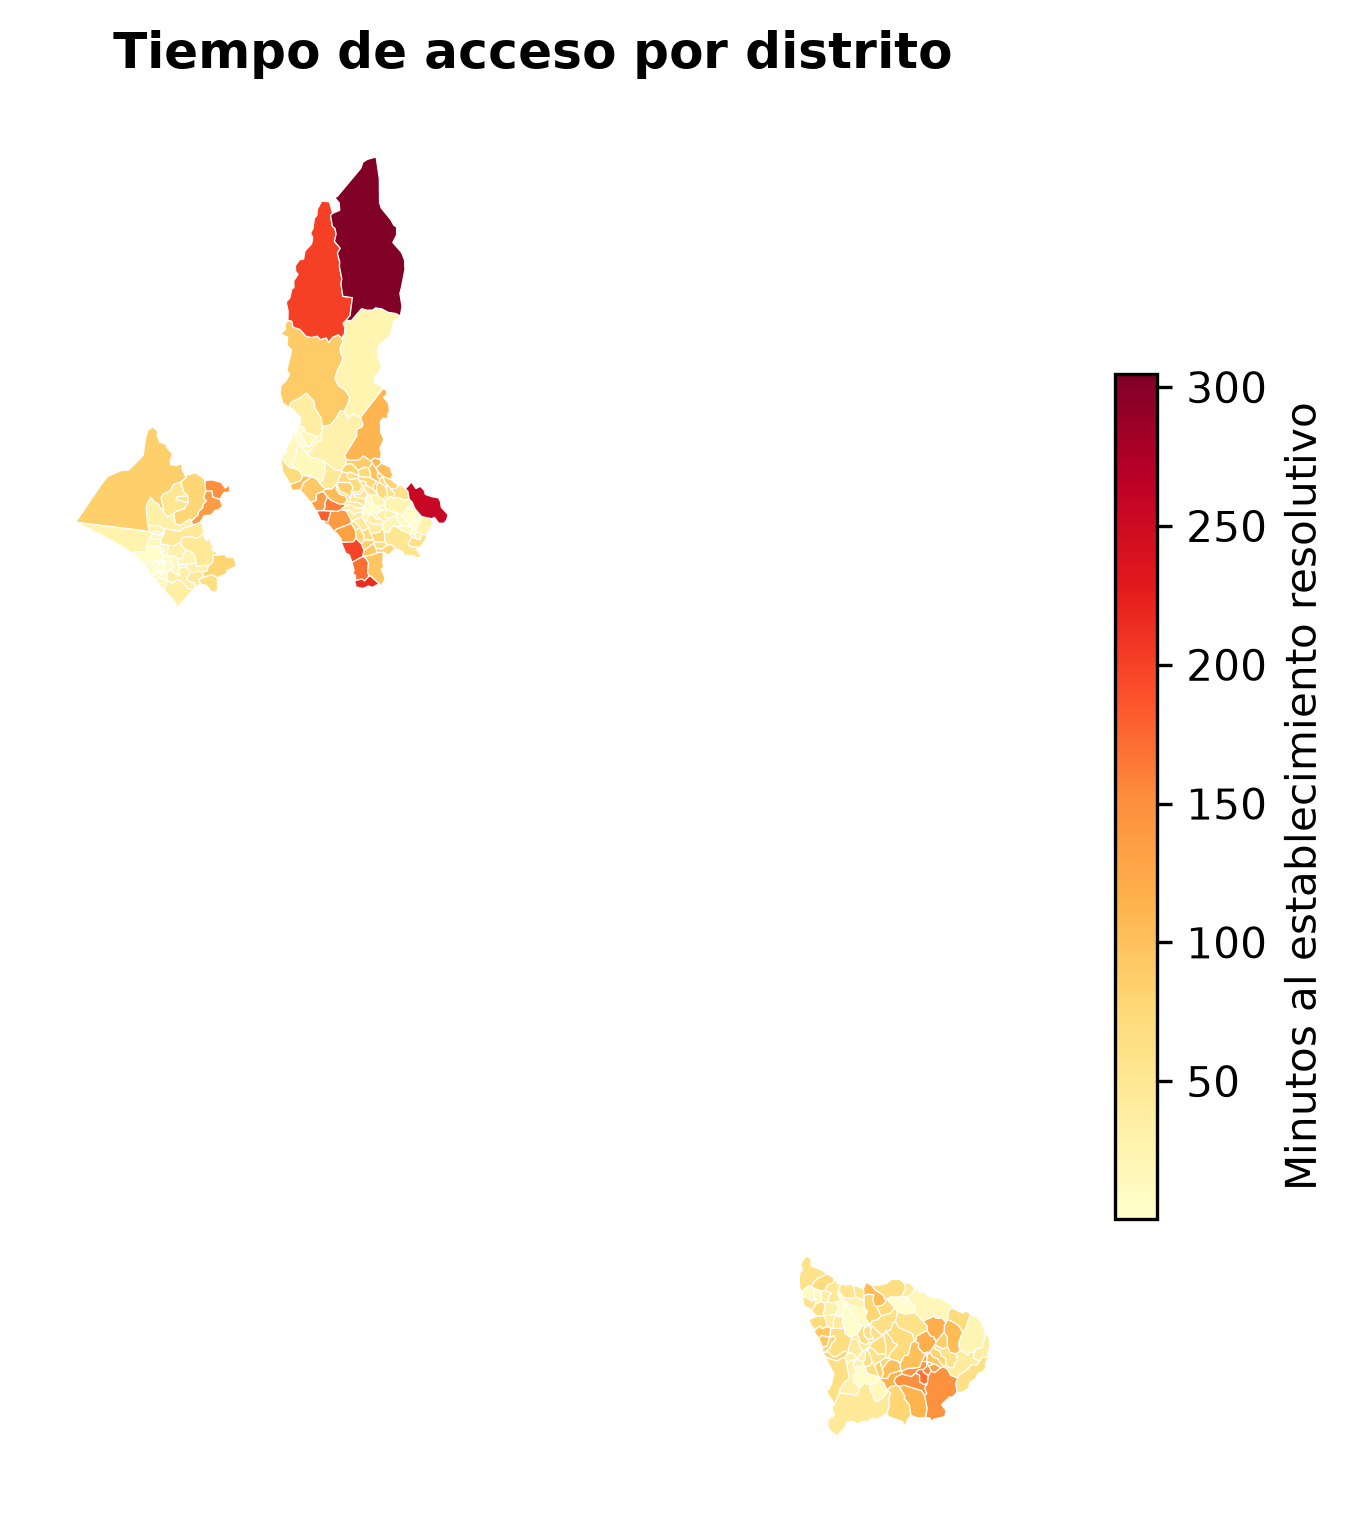
\includegraphics[width=0.62\linewidth]{fig_choropleth.png}
  \caption{Tiempo de acceso ponderado por poblaci\'on, por distrito.}
  \label{fig:choropleth}
\end{figure}

\begin{figure}[H]
  \centering
  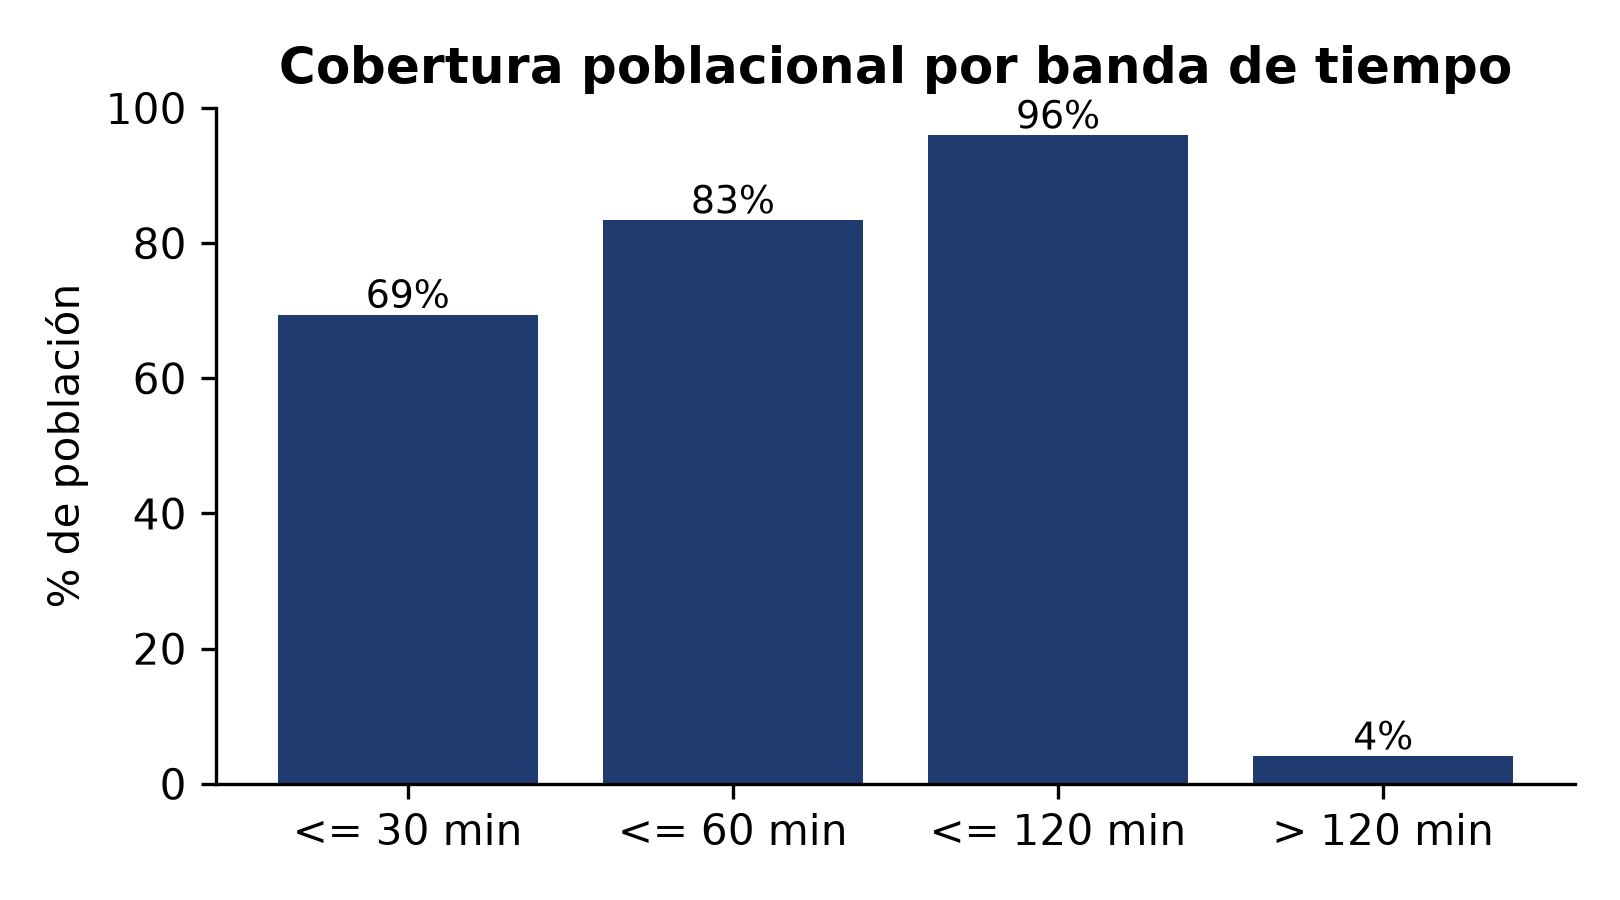
\includegraphics[width=0.49\linewidth]{fig_cobertura.png}\hfill
  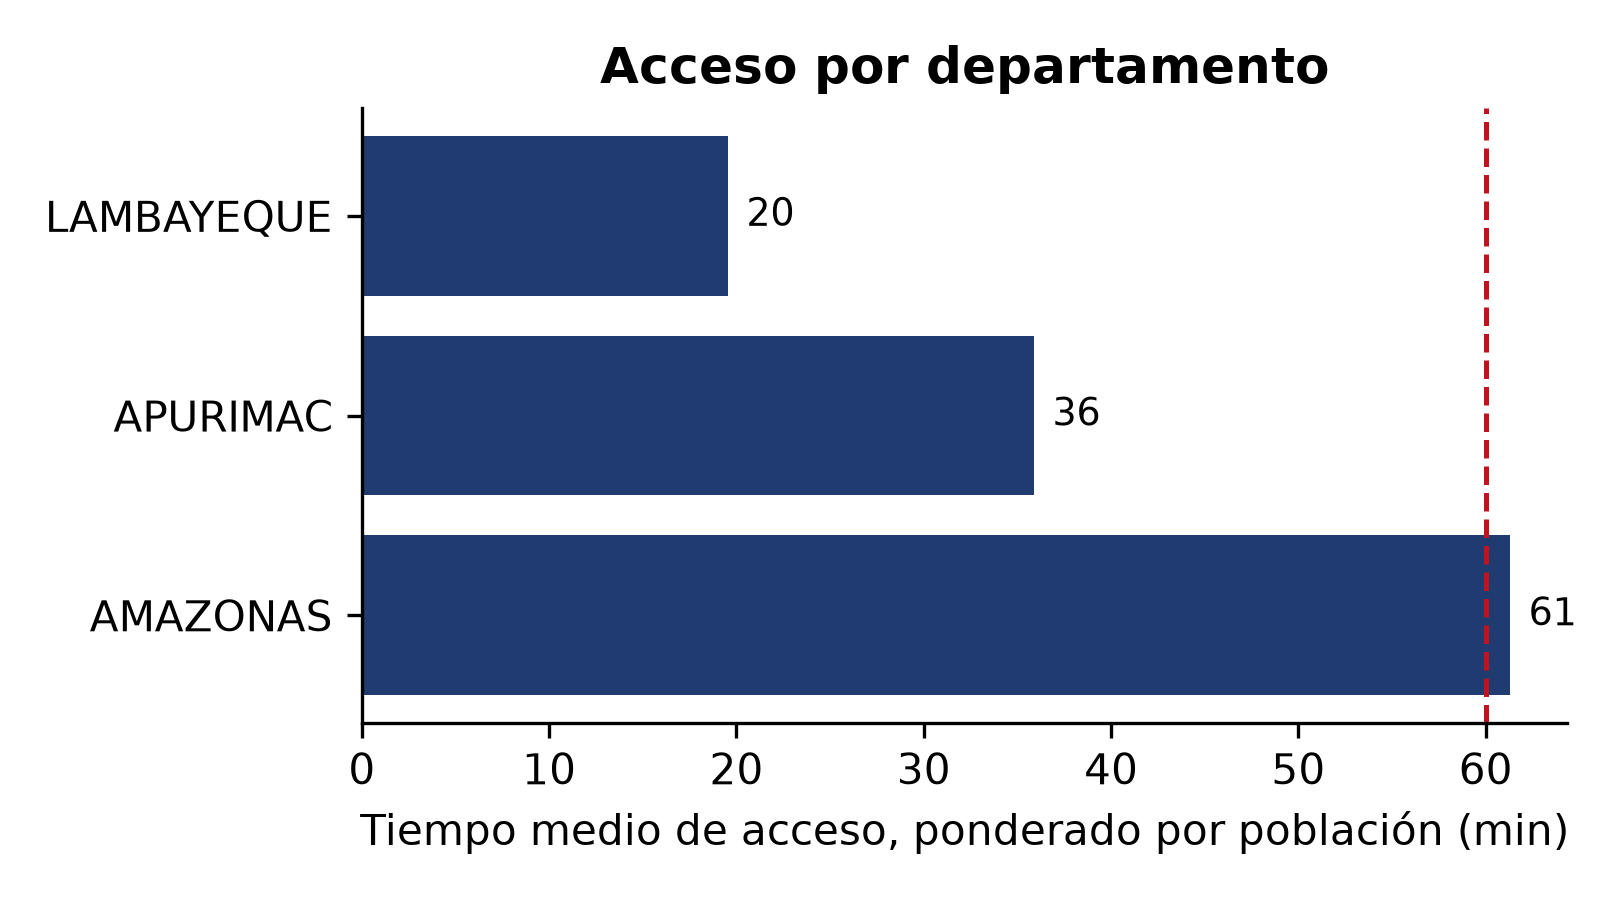
\includegraphics[width=0.49\linewidth]{fig_departamento.png}
  \caption{Izquierda: cobertura poblacional por banda de tiempo. Derecha: tiempo
  medio de acceso por departamento.}
  \label{fig:cobertura}
\end{figure}

\begin{figure}[H]
  \centering
  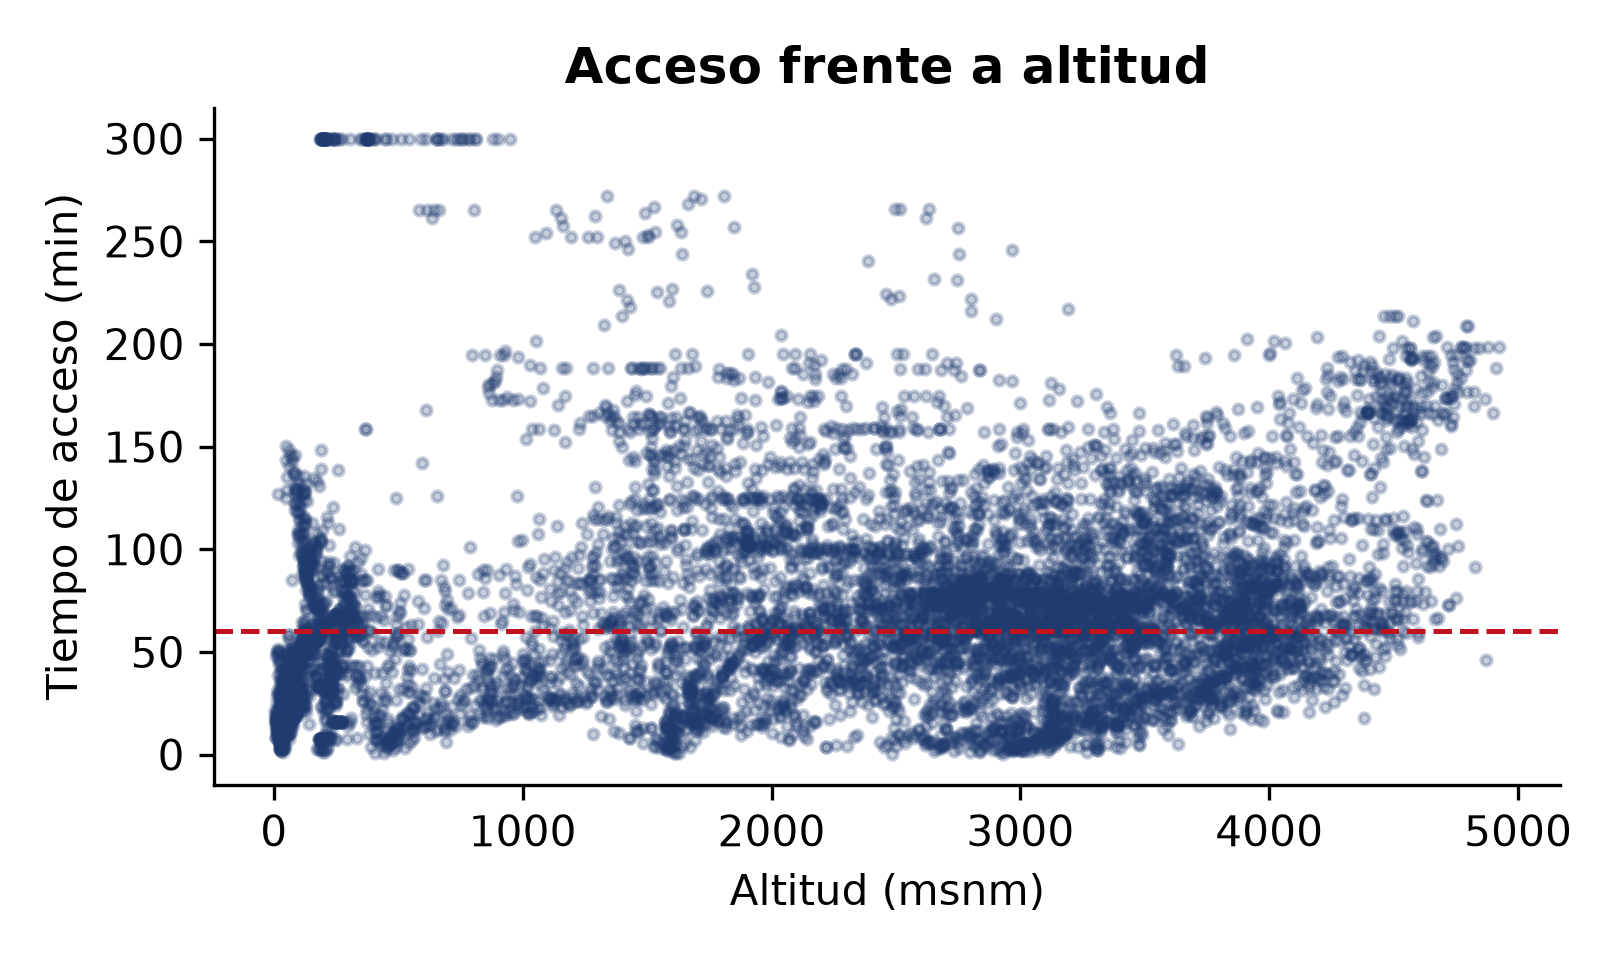
\includegraphics[width=0.72\linewidth]{fig_altitud.png}
  \caption{Tiempo de acceso frente a altitud del centro poblado.}
  \label{fig:altitud}
\end{figure}

\tab{tab_cobertura.tex}
\tab{tab_departamento.tex}
\tab{tab_distritos_peores.tex}

\paragraph{S\'intesis num\'erica} (perfil conducci\'on, ponderado por poblaci\'on;
fuente: \texttt{data/outputs/summary.json}).
\begin{itemize}
  \item Poblaci\'on del \'ambito: \num{1982403} habitantes en \num{8781} centros
        poblados; \num{39} establecimientos resolutivos.
  \item \textbf{Fuera de la hora dorada: \SI{16.6}{\percent}} de la poblaci\'on
        (\SI{4.1}{\percent} a m\'as de \num{120}~min). Cobertura acumulada:
        \SI{69.4}{\percent} a \num{30}~min, \SI{83.4}{\percent} a \num{60}~min.
  \item Tiempo medio ponderado \num{30.9}~min; mediana de centros poblados
        \num{63.8}~min: la poblaci\'on se concentra cerca de los hospitales,
        pero la mayor\'ia de localidades peque\~nas queda lejos.
  \item \textbf{Gini de acceso: \num{0.66}}.
  \item Urbano vs rural: \num{11.4}~min vs \num{62.9}~min.
  \item Por departamento: Lambayeque \num{19.5}~min (\SI{8.1}{\percent} fuera),
        Apur\'imac \num{35.9}~min (\SI{25.4}{\percent}), Amazonas
        \num{61.3}~min (\SI{34.2}{\percent}).
  \item Tercil de altitud (bajo/medio/alto): \numlist{25.2;39.9;57.4}~min.
  \item \textbf{Cuartil de pobreza distrital}: del menos al m\'as pobre,
        \numlist{15.5;47.0;58.1;113.2}~min. Correlaci\'on de $t_i$ con \% de
        pobreza $r=\num{0.35}$; con IDH $r=\num{-0.38}$.
  \item Comparaci\'on de perfiles: \num{30.9}~min en coche frente a
        \num{393}~min a pie (media ponderada) --- caminar no es una alternativa
        viable para la emergencia en este territorio.
\end{itemize}

\paragraph{Lectura de las figuras.}
La distribuci\'on del tiempo de acceso (Figura~\ref{fig:hist}) es fuertemente
asim\'etrica: una moda cerca de los \SI{20}{min} --- centros poblados
peri-urbanos --- y una cola larga que se extiende m\'as all\'a de las tres
horas. La diferencia entre la media ponderada (\num{30.9}~min) y la mediana de
centros poblados (\num{63.8}~min) resume el fen\'omeno: la poblaci\'on est\'a
concentrada en pocas localidades bien servidas, mientras que la mayor\'ia de
los n\'ucleos --- peque\~nos y dispersos --- quedan lejos. El
\emph{choropleth} (Figura~\ref{fig:choropleth}) localiza la carencia en el
norte de Amazonas: los distritos de la provincia de Condorcanqui
(\texttt{0104xx}) superan los \SI{200}{min}, y en varios de ellos el
\SI{100}{\percent} de la poblaci\'on queda fuera de la hora dorada
(Tabla~\ref{tab:peores}). Apur\'imac muestra un patr\'on m\'as homog\'eneo y
Lambayeque concentra el acceso r\'apido en el eje Chiclayo--Lambayeque. La
Figura~\ref{fig:cobertura} confirma el contraste entre departamentos, y la
Figura~\ref{fig:altitud} muestra que por encima de los \SI{2500}{msnm} apenas
hay centros poblados dentro de la hora dorada, aunque la relaci\'on no es
lineal: la altitud opera como \emph{proxy} de una red vial m\'as lenta y
sinuosa, no como causa directa.

\section{Discusi\'on}
\textbf{El problema no es de nivel medio sino de distribuci\'on.} Un tiempo
medio ponderado de \SI{31}{min} podr\'ia sugerir una situaci\'on aceptable,
pero el coeficiente de Gini de \num{0.66} --- comparable al de variables de
renta en contextos muy desiguales --- indica que ese promedio esconde
realidades opuestas: la poblaci\'on urbana costera resuelve el traslado en
minutos, mientras que cerca de \num{330} mil personas necesitan m\'as de una
hora y una fracci\'on relevante, m\'as de dos. Cualquier pol\'itica que se
gu\'ie por el promedio invisibiliza justamente a la poblaci\'on en riesgo.

\textbf{La brecha se alinea con la pobreza.} El resultado m\'as claro del
cruce con la dimensi\'on secundaria es el gradiente por cuartil de pobreza
distrital: del cuartil menos pobre al m\'as pobre, el tiempo medio de acceso
pasa de \SI{15}{min} a \SI{113}{min}, con una correlaci\'on positiva de
$t_i$ con el porcentaje de pobreza ($r=\num{0.35}$) y negativa con el IDH
($r=\num{-0.38}$). La carencia de acceso a emergencias no es independiente de
otras privaciones: se concentra donde ya hay menor renta, menor desarrollo
humano y --- t\'ipicamente --- menor densidad y peor infraestructura vial. El
acceso deficiente act\'ua as\'i como un multiplicador de desventajas
preexistentes.

\textbf{Regi\'on natural y ruralidad.} El orden costa\,$<$\,sierra\,$<$\,selva
(Lambayeque \SI{20}{min}, Apur\'imac \SI{36}{min}, Amazonas \SI{61}{min}) y el
contraste urbano/rural (\SI{11}{min} frente a \SI{63}{min}) apuntan a la misma
causa estructural: la resoluci\'on de emergencias se ha concentrado en las
capitales departamentales y provinciales, y la poblaci\'on rural amaz\'onica
--- con r\'ios como v\'ias principales y escasa red carrozable --- queda
sistem\'aticamente descubierta. El perfil peatonal (\num{393}~min de media)
descarta que caminar sea una alternativa: sin veh\'iculo, la hora dorada es
inalcanzable para casi toda la poblaci\'on fuera de las ciudades.

\textbf{Implicaciones.} El elevado Gini y la fuerte concentraci\'on espacial
de la carencia sugieren que \emph{unas pocas intervenciones bien localizadas}
--- elevar a categor\'ia resolutiva establecimientos ya existentes en
Condorcanqui, Bagua o las provincias altas de Apur\'imac --- reducir\'ian de
forma apreciable la poblaci\'on fuera de cobertura, mucho m\'as que un aumento
generalizado de recursos. El simulador del panel permite cuantificar cada
escenario: al a\~nadir un establecimiento resolutivo en un distrito
amaz\'onico desabastecido, el porcentaje de poblaci\'on fuera de la hora
dorada cae de forma visible. Este tipo de an\'alisis marginal es la
contribuci\'on pr\'actica del trabajo.

\section{Limitaciones}
Los resultados deben leerse como una estimaci\'on de referencia, no como un
tiempo de respuesta operativo. Las principales limitaciones son:

\begin{itemize}
  \item \textbf{Modelo est\'atico.} No se considera tr\'afico, hora del d\'ia,
        clima, estado del firme ni estacionalidad; en la selva, las crecidas
        pueden cortar v\'ias durante meses y elevar los tiempos reales muy por
        encima de lo estimado.
  \item \textbf{Traslado, no respuesta.} Se mide el trayecto vial origen--%
        destino; no se incluyen el tiempo de aviso, el despacho de la
        ambulancia, ni la posibilidad de traslado a\'ereo, que en algunas
        zonas amaz\'onicas es la \'unica v\'ia realista.
  \item \textbf{Cobertura de OSM.} La red vial est\'a menos completa en la
        selva; v\'ias no mapeadas producen sobrestimaci\'on del tiempo, y
        trochas de mala calidad mapeadas como v\'ias, subestimaci\'on.
  \item \textbf{Perfil peatonal aproximado.} Se deriva de la distancia vial a
        velocidad constante; es una cota comparativa, no un c\'alculo de rutas
        a pie.
  \item \textbf{Datos de 2017.} La poblaci\'on de centros poblados procede del
        \'ultimo censo y no capta la migraci\'on posterior.
  \item \textbf{Efectos de borde.} S\'olo se consideran establecimientos
        dentro de los tres departamentos; poblaci\'on cercana a un l\'imite
        podr\'ia tener m\'as cerca un hospital de la regi\'on vecina.
\end{itemize}

\section{Conclusiones}
Cerca de \num{330} mil personas (\SI{16.6}{\percent}) de Lambayeque, Apur\'imac y
Amazonas no pueden alcanzar un establecimiento de salud resolutivo dentro de la
hora dorada por carretera, y la carencia se concentra en la selva, en la altura
y --- de forma marcada --- en los distritos m\'as pobres, que tardan del orden de
siete veces m\'as que los menos pobres. El elevado coeficiente de Gini
(\num{0.66}) confirma que el problema no es un d\'eficit medio sino una
distribuci\'on muy desigual: bastar\'ia elevar a categor\'ia resolutiva unos
pocos establecimientos bien ubicados en la sierra y la selva para reducir de
forma apreciable la poblaci\'on fuera de cobertura, hip\'otesis que el simulador
del panel permite explorar.

\section*{Reproducibilidad}
C\'odigo y datos: \url{https://github.com/karelysscs/Practica_2_Data_Science}.
Todos los par\'ametros (departamentos, categor\'ias resolutivas, umbrales,
bandas) se declaran en \texttt{config.md}; el c\'odigo de \texttt{src/} no
contiene valores fijados. Ejecutar en orden:
\begin{verbatim}
python -m src.fase1_datos      # validacion + reportes de calidad
python -m src.fase2_ruteo      # matriz O-D via OSRM (cache reanudable)
python -m src.fase3_metricas   # metricas, Gini, cruces, GeoPackage
python -m src.fase5_figuras    # figuras .png y tablas .tex
streamlit run app.py           # panel interactivo
\end{verbatim}

\begin{thebibliography}{9}
\bibitem{golden} Lerner, E.B.; Moscati, R.M. (2001). The Golden Hour:
  scientific fact or medical urban legend? \emph{Acad. Emerg. Med.} 8(7).
\bibitem{osrm} Luxen, D.; Vetter, C. (2011). Real-time routing with
  OpenStreetMap data. \emph{ACM SIGSPATIAL GIS}.
\bibitem{renipress} SUSALUD. Registro Nacional de IPRESS (RENIPRESS), 2026.
\bibitem{inei} INEI. Censos Nacionales 2017: XII de Poblaci\'on y VII de
  Vivienda --- Centros Poblados.
\end{thebibliography}

\end{document}
